\subsubsection{Schritt 2: Kombination von Typ-Konvertierungsvarianten}\label{sem_eval_step2}
In diesem Schritt werden die ermittelten Typ-Konvertierungsvarianten miteinander kombiniert, was einer Kombination der angebotenen Interfaces gleicht. Die Anzahl $k$ der zu kombinierenden Typ-Konvertierungsvarianten kann jedoch variieren. Wenn $|EM|$ die Anzahl der Methoden im erwarteten Interface ist, gilt f�r $k$:
\begin{align*}
1 \leq k \leq |EM|
\end{align*}
\noindent
Da $k$ variabel ist, wird dieser Schritt zusammen mit allen folgenden Schritten mitunter mehrfach durchlaufen. Die Nummer des jeweiligen Iterationsschrittes wird mit $k$ gleichgesetzt. Somit wird die Anzahl der zu kombinierenden Typ-Konvertierungsvarianten mit jedem Durchlauf erh�ht. \abbref{tkv_alv_alu_1} zeigt die Kombinationen von Typ-Konvertierungsvarianten, die sich - bezogen auf die Beispiele aus \abbref{konvar_voll} und \abbref{konvar_unv} - im ersten Durchlauf ergeben. Im zweiten Durchlauf w�rde sich nur eine Kombination von Typ-Konvertierungsvarianten ergeben, da die beiden Typ-Konvertierungsvarianten von AIv und AIu miteinander kombiniert werden (siehe \abbref{comb_tkv_alv_alu_1}).



\begin{figure}[H]
\begin{minipage}[b]{.48\linewidth}
  \centering
  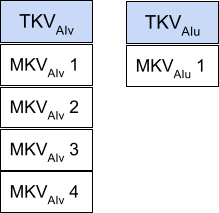
\includegraphics[width=.6\linewidth]{tkv_alv_alu_1}
  \caption{Kombinationen von Typ-Konvertierungsvarianten von AIu und AIv im ersten Durchlauf}
  \label{abb:tkv_alv_alu_1}

\end{minipage}%
\hspace{.04\linewidth}% Abstand zwischen Bilder
\begin{minipage}[b]{.48\linewidth}


  \centering
  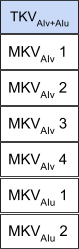
\includegraphics[width=.2\linewidth]{comb_tkv_alv_alu_1}
  \caption{Kombinationen von Typ-Konvertierungsvarianten von AIu und AIv im zweiten Durchlauf}
  \label{abb:comb_tkv_alv_alu_1}

\end{minipage}
\end{figure}

\noindent
So berechnet sich die Anzahl an ermittelten Kombinationen von Typ-Konvertierungsvarianten  ($|KombTKV|$) f�r jeden Durchlauf $k$ in Abh�ngigkeit von der Anzahl der in der 1. Stufe ermittelten Typ-Konvertierungsvarianten ($|TKV|$) wie folgt:
\begin{align*}
|KombTKV| = \frac{|TKV|! }{ (|TKV| - k)! * k!}
\end{align*}

